\documentclass[11pt]{article}
\usepackage[margin=18mm,headheight=22pt]{geometry}
\usepackage{amsmath}
\usepackage{fontspec}
\usepackage{unicode-math}
\setmainfont{NewCM10}[Extension=.otf,UprightFont=*-Book,BoldFont=*-Bold,ItalicFont=*-BookItalic,BoldItalicFont=*-BoldItalic]
\setsansfont{NewCMSans10}[Extension=.otf,UprightFont=*-Book,BoldFont=*-Bold,ItalicFont=*-BookOblique,BoldItalicFont=*-BoldOblique]
\setmathfont{NewCMMath-Book.otf}
\usepackage{xcolor}
\definecolor{FAUblue}{HTML}{04316A}
\definecolor{Paperblue}{HTML}{EEF2F7}
\definecolor{EEIgold}{HTML}{CC9C42}
\usepackage{etoolbox,enumitem,booktabs,tabularx,array,needspace,microtype}
\usepackage[most]{tcolorbox}
\usepackage{titlesec,fancyhdr}
\usepackage[hidelinks]{hyperref}
\usepackage{draftwatermark}
\SetWatermarkText{Made by Thanate Amornjiraporn (Focus)}
\SetWatermarkColor{black!7}\SetWatermarkFontSize{30pt}\SetWatermarkAngle{45}
\setlength{\parindent}{0pt}
\setlength{\parskip}{5pt}
\setlist{itemsep=2pt,topsep=3pt,leftmargin=1.6em,beginpenalty=10000,endpenalty=10000}
\raggedbottom
\clubpenalty=10000 \widowpenalty=10000 \displaywidowpenalty=10000 \interlinepenalty=10000
\setcounter{secnumdepth}{0}
\setcounter{tocdepth}{1}
\pagestyle{fancy}\fancyhf{}
\fancyhead[L]{\small\sffamily\color{FAUblue} From Fundamentals to AI Apocalypse · EEI · Tutorial 3}
\fancyhead[R]{\small\sffamily Tutorial 3: Worked solutions}
\fancyfoot[C]{\small\thepage}
\titleformat{\section}{\Large\bfseries\sffamily\color{FAUblue}}{}{0pt}{}
\titleformat{\subsection}{\large\bfseries\sffamily\color{FAUblue}}{}{0pt}{}
\titlespacing*{\section}{0pt}{16pt}{6pt}
\preto\section{\Needspace{8\baselineskip}}
\preto\subsection{\Needspace{6\baselineskip}}
\newtcolorbox{equationcard}[1]{colback=Paperblue,colframe=Paperblue,boxrule=0pt,arc=0pt,left=10pt,right=10pt,top=6pt,bottom=6pt,title={#1},fonttitle=\small\bfseries\sffamily,coltitle=FAUblue,before skip=8pt,after skip=8pt}
\newtcolorbox{workedbox}[1]{colback=white,colframe=EEIgold,boxrule=0pt,leftrule=3pt,arc=0pt,left=10pt,top=4pt,bottom=4pt,title={#1},fonttitle=\small\bfseries\sffamily,coltitle=FAUblue,attach title to upper={\par},before skip=8pt,after skip=8pt}
\newtcolorbox{recallbox}[1]{colback=white,colframe=FAUblue,boxrule=0pt,leftrule=3pt,arc=0pt,left=10pt,top=4pt,bottom=4pt,title={#1},fonttitle=\small\bfseries\sffamily,coltitle=FAUblue,attach title to upper={\par},before skip=8pt,after skip=8pt}
\usepackage{environ}
\newsavebox\measurebox
% Typeset the section once invisibly to measure it; start a new page if it will not fit in what is left.
\makeatletter
\newif\ifkeep@measuring
\NewEnviron{keepsection}{%
  \ifkeep@measuring \BODY \else
    \edef\keep@sec{\the\value{section}}\edef\keep@sub{\the\value{subsection}}%
    \setbox\measurebox\vbox{\hsize\linewidth\keep@measuringtrue\def\Needspace##1{}\BODY}%
    \setcounter{section}{\keep@sec}\setcounter{subsection}{\keep@sub}%
    \dimen2=\ht\measurebox \advance\dimen2\dp\measurebox
    \dimen@=\textheight
    \ifdim\pagegoal<\maxdimen
      \dimen@=\pagegoal \advance\dimen@-\pagetotal
      \ifdim\dimen2>\dimen@ \clearpage \dimen@=\textheight \fi
    \fi
    % if it fits, nothing inside may force an early break
    \ifdim\dimen2>\dimen@ \BODY \else \begingroup\def\Needspace##1{}\BODY\endgroup \fi
  \fi}
\makeatother
\newtcolorbox{notebox}{colback=Paperblue,colframe=Paperblue,boxrule=0pt,arc=0pt,left=8pt,right=8pt,top=4pt,bottom=4pt,before skip=6pt,after skip=6pt}
\newtcolorbox{plainbox}{colback=white,colframe=FAUblue,boxrule=0pt,leftrule=3pt,arc=0pt,left=10pt,right=8pt,top=4pt,bottom=4pt,before skip=6pt,after skip=8pt}
\usetikzlibrary{arrows.meta}
\title{\sffamily\bfseries\color{FAUblue}Tutorial 3: Worked solutions}
\author{Electrical Engineering I \ensuremath{\cdot} Module 92315 \ensuremath{\cdot} Tutorial 3\\[2pt]\small From Fundamentals to AI Apocalypse · personal study guide}
\date{}
\begin{document}
\maketitle
\begingroup\footnotesize\setlength{\parskip}{0pt}\tableofcontents\endgroup
\clearpage

\Needspace{9\baselineskip}
{\large Resolve each interaction from its geometry, then add force vectors component by component. In Task 7, use Newton’s third law to separate the known pair interaction from the supplied net forces.}


\begin{keepsection}
\Needspace{11\baselineskip}
\section{Task 6: Line and point charges}

\Needspace{8\baselineskip}
Use the shown xy cross-section: Q\textsubscript{1} = (\ensuremath{-}a, 0), Q\textsubscript{2} = (a, 0), the line λ\textsubscript{1} passes through (0, a), and λ\textsubscript{2} passes through (0, \ensuremath{-}a/2). Both lines run parallel to z. Take air as vacuum for the field formulas, as instructed, and assume a \ensuremath{>} 0.

\Needspace{11\baselineskip}
\textbf{Connected topic:} Electric field strength (§1.3) gives Coulomb’s field and vector superposition. The line-charge formula is applied with its radial direction converted to Cartesian components.

\Needspace{14\baselineskip}
\begin{center}
\begin{minipage}[t]{0.950\linewidth}\centering
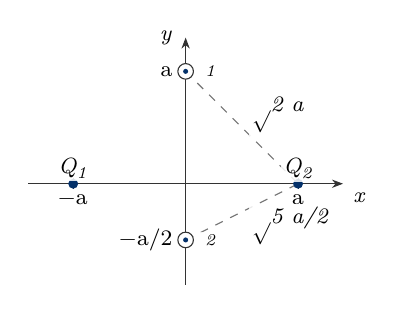
\begin{tikzpicture}[line join=round]
\draw[-{Stealth[length=4pt]},black!80] (0.503,-2.359) -- (4.501,-2.359);
\node[anchor=west,fill=white,fill opacity=0.85,text opacity=1,inner sep=1pt,font=\footnotesize] at (4.591,-2.539) {\textit{x}};
\draw[-{Stealth[length=4pt]},black!80] (2.502,-3.644) -- (2.502,-0.503);
\node[anchor=east,fill=white,fill opacity=0.85,text opacity=1,inner sep=1pt,font=\footnotesize] at (2.376,-0.503) {\textit{y}};
\draw[black!80] (1.074,-2.287) -- (1.074,-2.431);
\node[fill=white,fill opacity=0.85,text opacity=1,inner sep=1pt,font=\footnotesize] at (1.074,-2.557) {\ensuremath{-}a};
\draw[black!80] (3.930,-2.287) -- (3.930,-2.431);
\node[fill=white,fill opacity=0.85,text opacity=1,inner sep=1pt,font=\footnotesize] at (3.930,-2.557) {a};
\draw[black!80] (2.430,-0.932) -- (2.574,-0.932);
\node[anchor=east,fill=white,fill opacity=0.85,text opacity=1,inner sep=1pt,font=\footnotesize] at (2.376,-0.932) {a};
\draw[black!80] (2.430,-3.073) -- (2.574,-3.073);
\node[anchor=east,fill=white,fill opacity=0.85,text opacity=1,inner sep=1pt,font=\footnotesize] at (2.376,-3.073) {\ensuremath{-}a/2};
\draw[black!55,dashed] (2.502,-0.932) -- (3.930,-2.359);
\draw[black!55,dashed] (2.502,-3.073) -- (3.930,-2.359);
\node[anchor=west,fill=white,fill opacity=0.85,text opacity=1,inner sep=1pt,font=\footnotesize] at (3.306,-1.483) {\textit{\ensuremath{\surd}2 a}};
\node[anchor=west,fill=white,fill opacity=0.85,text opacity=1,inner sep=1pt,font=\footnotesize] at (3.306,-2.896) {\textit{\ensuremath{\surd}5 a/2}};
\fill[FAUblue] (1.074,-2.359) circle (0.063);
\node[fill=white,fill opacity=0.85,text opacity=1,inner sep=1pt,font=\footnotesize] at (1.074,-2.161) {\textit{Q\textsubscript{1}}};
\fill[FAUblue] (3.930,-2.359) circle (0.063);
\node[fill=white,fill opacity=0.85,text opacity=1,inner sep=1pt,font=\footnotesize] at (3.930,-2.161) {\textit{Q\textsubscript{2}}};
\filldraw[draw=black!80,fill=white] (2.502,-0.932) circle (0.099);
\fill[FAUblue] (2.502,-0.932) circle (0.032);
\node[anchor=west,fill=white,fill opacity=0.85,text opacity=1,inner sep=1pt,font=\footnotesize] at (2.628,-0.932) {\textit{λ\textsubscript{1}}};
\filldraw[draw=black!80,fill=white] (2.502,-3.073) circle (0.099);
\fill[FAUblue] (2.502,-3.073) circle (0.032);
\node[anchor=west,fill=white,fill opacity=0.85,text opacity=1,inner sep=1pt,font=\footnotesize] at (2.628,-3.073) {\textit{λ\textsubscript{2}}};
\end{tikzpicture}\par\smallskip{\small\raggedright \textbf{Distances to Q\textsubscript{2}.} The point charges sit on the x-axis at \ensuremath{\pm}\textit{a}; the line charges run along z through (0, \textit{a}) and (0, \ensuremath{-}\textit{a}/2). The dashed lines are the perpendicular distances from each line to Q\textsubscript{2}, \ensuremath{\sqrt{2}} \textit{a} and \ensuremath{\sqrt{5}} \textit{a}/2, which set the line fields there.\par}\end{minipage}
\end{center}

\begin{keepsection}
\Needspace{7\baselineskip}
\subsection{6a: Field of Q\textsubscript{1} at Q\textsubscript{2}}

\Needspace{4\baselineskip}
Try first: find the displacement from Q\textsubscript{1} to Q\textsubscript{2}, then use Coulomb’s field with that direction and distance.

\nopagebreak[4]{\small\itshape Answers: see “Task 6: Line and point charges” under Answers at the end.}
\end{keepsection}

\begin{keepsection}
\Needspace{6\baselineskip}
\subsection{6b: Force of Q\textsubscript{1} on Q\textsubscript{2}}

\Needspace{3\baselineskip}
Try first: multiply the field from 6a by the charge that experiences it, Q\textsubscript{2}.

\nopagebreak[4]{\small\itshape Answers: see “Task 6: Line and point charges” under Answers at the end.}
\end{keepsection}

\begin{keepsection}
\Needspace{7\baselineskip}
\subsection{6c: Field of λ\textsubscript{1} and λ\textsubscript{2} at Q\textsubscript{2}}

\Needspace{4\baselineskip}
Try first: form the transverse displacement from each line to Q\textsubscript{2}, normalize it, and add the two line fields.

\nopagebreak[4]{\small\itshape Answers: see “Task 6: Line and point charges” under Answers at the end.}
\end{keepsection}

\begin{keepsection}
\Needspace{6\baselineskip}
\subsection{6d: Force of the lines on Q\textsubscript{2}}

\Needspace{3\baselineskip}
Try first: use the field sum from 6c and multiply by Q\textsubscript{2}.

\nopagebreak[4]{\small\itshape Answers: see “Task 6: Line and point charges” under Answers at the end.}
\end{keepsection}

\begin{keepsection}
\Needspace{7\baselineskip}
\subsection{6e: Total force on Q\textsubscript{2}}

\Needspace{4\baselineskip}
Try first: add the point-charge force from 6b to the line-charge force from 6d, keeping x and y components separate.

\nopagebreak[4]{\small\itshape Answers: see “Task 6: Line and point charges” under Answers at the end.}
\end{keepsection}

\begin{keepsection}
\Needspace{6\baselineskip}
\subsection{6f: Condition for zero total force}

\Needspace{3\baselineskip}
Try first: set both components from 6e to zero and solve the y equation before the x equation.

\nopagebreak[4]{\small\itshape Answers: see “Task 6: Line and point charges” under Answers at the end.}
\end{keepsection}
\end{keepsection}

\begin{keepsection}
\Needspace{11\baselineskip}
\section{Task 7: Point charge}

\Needspace{8\baselineskip}
Take Q \ensuremath{>} 0 as the reference scale. The figure places Q\textsubscript{1} = \ensuremath{\sqrt{5}} Q at (0, a) and Q\textsubscript{2} = \ensuremath{\sqrt{2}} Q at (3a, 0). The supplied net forces on Q\textsubscript{1} and Q\textsubscript{2} are F\textsubscript{1} = F\textsubscript{0}[\ensuremath{-}(3 + 5\ensuremath{\sqrt{5}})e\textsubscript{x} + e\textsubscript{y}] and F\textsubscript{2} = F\textsubscript{0}(13e\textsubscript{x} \ensuremath{-} 11e\textsubscript{y}), with F\textsubscript{0} = Q²/(40πε\textsubscript{0}a²). The charges are in vacuum and a \ensuremath{>} 0; F\textsubscript{0} is a force scale measured in newtons.

\Needspace{9\baselineskip}
\textbf{Connected topic:} Electric field strength (§1.3) connects Coulomb force, displacement direction and vector superposition.

\Needspace{14\baselineskip}
\begin{center}
\begin{minipage}[t]{0.950\linewidth}\centering
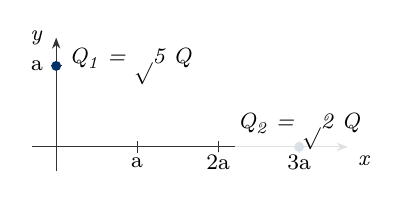
\begin{tikzpicture}[line join=round]
\draw[-{Stealth[length=4pt]},black!80] (0.586,-1.923) -- (4.598,-1.923);
\node[anchor=west,fill=white,fill opacity=0.85,text opacity=1,inner sep=1pt,font=\footnotesize] at (4.688,-2.103) {\textit{x}};
\draw[-{Stealth[length=4pt]},black!80] (0.895,-2.232) -- (0.895,-0.535);
\node[anchor=east,fill=white,fill opacity=0.85,text opacity=1,inner sep=1pt,font=\footnotesize] at (0.769,-0.535) {\textit{y}};
\draw[black!80] (1.923,-1.851) -- (1.923,-1.995);
\node[fill=white,fill opacity=0.85,text opacity=1,inner sep=1pt,font=\footnotesize] at (1.923,-2.121) {a};
\draw[black!80] (2.952,-1.851) -- (2.952,-1.995);
\node[fill=white,fill opacity=0.85,text opacity=1,inner sep=1pt,font=\footnotesize] at (2.952,-2.121) {2a};
\draw[black!80] (3.981,-1.851) -- (3.981,-1.995);
\node[fill=white,fill opacity=0.85,text opacity=1,inner sep=1pt,font=\footnotesize] at (3.981,-2.121) {3a};
\draw[black!80] (0.823,-0.895) -- (0.967,-0.895);
\node[anchor=east,fill=white,fill opacity=0.85,text opacity=1,inner sep=1pt,font=\footnotesize] at (0.769,-0.895) {a};
\fill[FAUblue] (0.895,-0.895) circle (0.063);
\node[anchor=west,fill=white,fill opacity=0.85,text opacity=1,inner sep=1pt,font=\footnotesize] at (1.021,-0.895) {\textit{Q\textsubscript{1} = \ensuremath{\surd}5 Q}};
\fill[FAUblue] (3.981,-1.923) circle (0.063);
\node[fill=white,fill opacity=0.85,text opacity=1,inner sep=1pt,font=\footnotesize] at (3.981,-1.725) {\textit{Q\textsubscript{2} = \ensuremath{\surd}2 Q}};
\end{tikzpicture}\par\smallskip{\small\raggedright \textbf{The two known charges.} Q\textsubscript{1} = \ensuremath{\sqrt{5}} Q sits at (0, \textit{a}) and Q\textsubscript{2} = \ensuremath{\sqrt{2}} Q at (3\textit{a}, 0). The third charge is not drawn: its position is what 7e finds from the directions of the forces.\par}\end{minipage}
\end{center}

\begin{keepsection}
\Needspace{7\baselineskip}
\subsection{7a: Force F\textsubscript{12} of Q\textsubscript{2} on Q\textsubscript{1}}

\Needspace{4\baselineskip}
Try first: find the vector from Q\textsubscript{2} to Q\textsubscript{1} and substitute both charges and their separation into Coulomb’s law.

\nopagebreak[4]{\small\itshape Answers: see “Task 7: Point charge” under Answers at the end.}
\end{keepsection}

\begin{keepsection}
\Needspace{6\baselineskip}
\subsection{7b: Force F\textsubscript{21} of Q\textsubscript{1} on Q\textsubscript{2}}

\Needspace{3\baselineskip}
Try first: use Newton’s third law for the same pair.

\nopagebreak[4]{\small\itshape Answers: see “Task 7: Point charge” under Answers at the end.}
\end{keepsection}

\begin{keepsection}
\Needspace{6\baselineskip}
\subsection{7c: Force F\textsubscript{13} of Q\textsubscript{3} on Q\textsubscript{1}}

\Needspace{3\baselineskip}
Try first: subtract the known Q\textsubscript{2} contribution from the supplied net force on Q\textsubscript{1}.

\nopagebreak[4]{\small\itshape Answers: see “Task 7: Point charge” under Answers at the end.}
\end{keepsection}

\begin{keepsection}
\Needspace{6\baselineskip}
\subsection{7d: Force F\textsubscript{23} of Q\textsubscript{3} on Q\textsubscript{2}}

\Needspace{3\baselineskip}
Try first: add F\textsubscript{12} to the net force on Q\textsubscript{2}, using F\textsubscript{21} = \ensuremath{-}F\textsubscript{12}.

\nopagebreak[4]{\small\itshape Answers: see “Task 7: Point charge” under Answers at the end.}
\end{keepsection}

\begin{keepsection}
\Needspace{7\baselineskip}
\subsection{7e: Coordinates of Q\textsubscript{3}}

\Needspace{4\baselineskip}
Try first: intersect the horizontal line through Q\textsubscript{1} with the diagonal direction line through Q\textsubscript{2}.

\nopagebreak[4]{\small\itshape Answers: see “Task 7: Point charge” under Answers at the end.}
\end{keepsection}

\begin{keepsection}
\Needspace{6\baselineskip}
\subsection{7f: Charge ratio Q\textsubscript{3}/Q}

\Needspace{3\baselineskip}
Try first: use the magnitude of F\textsubscript{13}, the separation 2a, and Q\textsubscript{1} = \ensuremath{\sqrt{5}} Q.

\nopagebreak[4]{\small\itshape Answers: see “Task 7: Point charge” under Answers at the end.}
\end{keepsection}

\begin{keepsection}
\Needspace{6\baselineskip}
\subsection{7g: Total force F\textsubscript{3} on Q\textsubscript{3}}

\Needspace{3\baselineskip}
Try first: reverse F\textsubscript{13} and F\textsubscript{23} by Newton’s third law, then add them.

\nopagebreak[4]{\small\itshape Answers: see “Task 7: Point charge” under Answers at the end.}
\end{keepsection}
\end{keepsection}


\clearpage
\section{Answers}
\begin{keepsection}\subsection{Task 6: Line and point charges}

\begin{workedbox}{6a \ensuremath{\cdot} Point-charge field}
\Needspace{7\baselineskip}
\begin{enumerate}
\item \Needspace{5\baselineskip}
The source is at x = \ensuremath{-}a and the field point at x = a, so the displacement points along +x and has length 2a:

\begin{equation*}{R}_{21}\, =\, 2{a}\, {e}_{\mathrm{x}},\quad \, \quad \, |{R}_{21}|\, =\, 2{a}\end{equation*}
\item \Needspace{4\baselineskip}
Coulomb’s field is the source charge times the radial unit vector divided by 4πε\textsubscript{0}R²:

\Needspace{4\baselineskip}
\begin{equation*}{E}_{\mathrm{Q}1}({Q}_{2})\, =\, \dfrac{{Q}_{1}}{4πε_{0}\, |{R}_{21}|^{2}}\, {e}_{\mathrm{x}}\end{equation*}

\Needspace{4\baselineskip}
\begin{equation*}{E}_{\mathrm{Q}1}({Q}_{2})\, =\, \dfrac{{Q}_{1}}{16πε_{0}\, {a}^{2}}\, {e}_{\mathrm{x}}\end{equation*}

The sign of Q\textsubscript{1} sets whether the field points +x or \ensuremath{-}x. The 1/(2a)² factor is easy to miss.
\end{enumerate}
\end{workedbox}

\end{keepsection}
\begin{keepsection}\subsection{Task 6: Line and point charges}

\begin{workedbox}{6b \ensuremath{\cdot} Point-charge force}
\Needspace{6\baselineskip}
\begin{enumerate}
\item \Needspace{4\baselineskip}
The electric force on a charge is its charge times the electric field at its position:

\begin{equation*}{F}_{12}\, =\, {Q}_{2}\, {E}_{\mathrm{Q}1}({Q}_{2})\end{equation*}
\item \Needspace{4\baselineskip}
Substitute the result from 6a:

\Needspace{5\baselineskip}
\begin{equation*}{F}_{12}\, =\, \dfrac{{Q}_{1}\, {Q}_{2}}{16πε_{0}\, {a}^{2}}\, {e}_{\mathrm{x}}\end{equation*}

Like signs give a force toward +x on Q\textsubscript{2}; opposite signs reverse it. Its units are newtons because charge times field is C\ensuremath{\cdot}N/C.
\end{enumerate}
\end{workedbox}

\end{keepsection}
\begin{keepsection}\subsection{Task 6: Line and point charges}

\begin{workedbox}{6c \ensuremath{\cdot} Infinite-line fields}
\Needspace{9\baselineskip}
\begin{enumerate}
\item \Needspace{5\baselineskip}
For λ\textsubscript{1}, the displacement from its axis (0, a) to Q\textsubscript{2} (a, 0) is (a, \ensuremath{-}a). Its radius is \ensuremath{\sqrt{2}} a and its radial unit vector is (e\textsubscript{x} \ensuremath{-} e\textsubscript{y})/\ensuremath{\sqrt{2}}:

\begin{equation*}{E}_{λ1}\, =\, \dfrac{λ_{1}}{2πε_{0}\, \sqrt{2}\, {a}}\, \cdot \, \dfrac{{e}_{\mathrm{x}}\, -\, {e}_{\mathrm{y}}}{\sqrt{2}}\, =\, \dfrac{λ_{1}}{4πε_{0}\, {a}}({e}_{\mathrm{x}}\, -\, {e}_{\mathrm{y}})\end{equation*}
\item \Needspace{4\baselineskip}
For λ\textsubscript{2}, the displacement is (a, a/2), with radius \ensuremath{\sqrt{5}} a/2 and unit direction (2e\textsubscript{x} + e\textsubscript{y})/\ensuremath{\sqrt{5}}:

\begin{equation*}{E}_{λ2}\, =\, \dfrac{λ_{2}}{πε_{0}\, \sqrt{5}\, {a}}\, \cdot \, \dfrac{2{e}_{\mathrm{x}}\, +\, {e}_{\mathrm{y}}}{\sqrt{5}}\, =\, \dfrac{λ_{2}}{5πε_{0}\, {a}}(2{e}_{\mathrm{x}}\, +\, {e}_{\mathrm{y}})\end{equation*}
\item \Needspace{4\baselineskip}
Add the x and y components separately:

\Needspace{5\baselineskip}
\begin{equation*}{E}_{\text{lines}}\, =\, \dfrac{1}{πε_{0}\, {a}}\left[\left(\dfrac{λ_{1}}{4}\, +\, \dfrac{2λ_{2}}{5}\right){e}_{\mathrm{x}}\, +\, \left(-\dfrac{λ_{1}}{4}\, +\, \dfrac{λ_{2}}{5}\right){e}_{\mathrm{y}}\right]\end{equation*}

Check the second line’s distance is a\ensuremath{\sqrt{5}}/2, not a\ensuremath{\sqrt{5}}; its source is only a/2 below the x-axis. Each field component has units N/C.
\end{enumerate}
\end{workedbox}

\end{keepsection}
\begin{keepsection}\subsection{Task 6: Line and point charges}

\begin{workedbox}{6d \ensuremath{\cdot} Force from both lines}
\Needspace{6\baselineskip}
\begin{enumerate}
\item \Needspace{4\baselineskip}
Both line fields act at Q\textsubscript{2}, so their combined force is Q\textsubscript{2} times their vector sum:

\begin{equation*}{F}_{\text{lines},2}\, =\, {Q}_{2}\, {E}_{\text{lines}}\end{equation*}
\item \Needspace{4\baselineskip}
Therefore:

\Needspace{5\baselineskip}
\begin{equation*}{F}_{\text{lines},2}\, =\, \dfrac{{Q}_{2}}{πε_{0}\, {a}}\left[\left(\dfrac{λ_{1}}{4}\, +\, \dfrac{2λ_{2}}{5}\right){e}_{\mathrm{x}}\, +\, \left(-\dfrac{λ_{1}}{4}\, +\, \dfrac{λ_{2}}{5}\right){e}_{\mathrm{y}}\right]\end{equation*}

A negative component indicates the corresponding force points along the negative axis; the force components are in newtons.
\end{enumerate}
\end{workedbox}

\end{keepsection}
\begin{keepsection}\subsection{Task 6: Line and point charges}

\begin{workedbox}{6e \ensuremath{\cdot} Superposition of all forces}
\Needspace{7\baselineskip}
\begin{enumerate}
\item \Needspace{5\baselineskip}
Electrostatic forces add linearly, so the total is the point-charge contribution plus the two-line contribution:

\begin{equation*}{F}_{2}\, =\, {F}_{12}\, +\, {F}_{\text{lines},2}\end{equation*}
\item \Needspace{4\baselineskip}
Collect the coefficients of each Cartesian direction:

\Needspace{4\baselineskip}
\begin{equation*}{F}_{2}\, =\, \left[\dfrac{{Q}_{1}\, {Q}_{2}}{16πε_{0}\, {a}^{2}}\, +\, \dfrac{{Q}_{2}}{πε_{0}\, {a}}\left(\dfrac{λ_{1}}{4}\, +\, \dfrac{2λ_{2}}{5}\right)\right]{e}_{\mathrm{x}}\, +\, \dfrac{{Q}_{2}}{πε_{0}\, {a}}\left(-\dfrac{λ_{1}}{4}\, +\, \dfrac{λ_{2}}{5}\right){e}_{\mathrm{y}}\end{equation*}

\textbf{Check:} if both line densities vanish, this reduces to the Coulomb force in 6b.
\end{enumerate}
\end{workedbox}

\end{keepsection}
\begin{keepsection}\subsection{Task 6: Line and point charges}

\begin{workedbox}{6f \ensuremath{\cdot} Balance the two components}
\Needspace{7\baselineskip}
\begin{enumerate}
\item \Needspace{4\baselineskip}
Q\textsubscript{2} is nonzero, so the y-component vanishes when:

\begin{equation*}-\dfrac{λ_{1}}{4}\, +\, \dfrac{λ_{2}}{5}\, =\, 0\, \quad \, \quad \Rightarrow \quad \, \quad \, λ_{2}\, =\, \dfrac{5λ_{1}}{4}\end{equation*}
\item \Needspace{4\baselineskip}
Insert this relation into the x-component, including the field from Q\textsubscript{1}:

\Needspace{4\baselineskip}
\begin{equation*}\dfrac{{Q}_{1}}{16{a}^{2}}\, +\, \dfrac{λ_{1}}{4{a}}\, +\, \dfrac{2}{5{a}}\, \cdot \, \dfrac{5λ_{1}}{4}\, =\, 0\end{equation*}

\begin{equation*}\dfrac{{Q}_{1}}{16{a}^{2}}\, +\, \dfrac{3λ_{1}}{4{a}}\, =\, 0\, \quad \, \quad \Rightarrow \quad \, \quad \, {Q}_{1}\, =\, -12{a}λ_{1}\end{equation*}
\item Thus the required condition is \textbf{λ\textsubscript{2} = 5λ\textsubscript{1}/4 and Q\textsubscript{1} = \ensuremath{-}12aλ\textsubscript{1}} (equivalently λ\textsubscript{1} = \ensuremath{-}Q\textsubscript{1}/(12a), λ\textsubscript{2} = \ensuremath{-}5Q\textsubscript{1}/(48a)). These signs make the line forces cancel in y and balance Q\textsubscript{1}’s x contribution.
\end{enumerate}
\end{workedbox}

\end{keepsection}
\begin{keepsection}\subsection{Task 7: Point charge}

\begin{workedbox}{7a \ensuremath{\cdot} First known pair force}
\Needspace{8\baselineskip}
\begin{enumerate}
\item \Needspace{4\baselineskip}
The displacement from Q\textsubscript{2} at (3a, 0) to Q\textsubscript{1} at (0, a) is (\ensuremath{-}3a, a), and the distance is \ensuremath{\sqrt{10}} a:

\begin{equation*}{R}_{12}\, =\, {a}(-3{e}_{\mathrm{x}}\, +\, {e}_{\mathrm{y}}),\quad \, \quad \, |{R}_{12}|\, =\, \sqrt{10}\, {a}\end{equation*}
\item \Needspace{5\baselineskip}
Coulomb force on Q\textsubscript{1} from Q\textsubscript{2} is kQ\textsubscript{1}Q\textsubscript{2} times the unit displacement divided by R². Here Q\textsubscript{1}Q\textsubscript{2} = \ensuremath{\sqrt{10}} Q²:

\Needspace{4\baselineskip}
\begin{equation*}{F}_{12}\, =\, \dfrac{1}{4πε_{0}}\, \cdot \, \dfrac{{Q}_{1}\, {Q}_{2}}{|{R}_{12}|^{3}}\, {R}_{12}\, =\, \dfrac{1}{4πε_{0}}\, \cdot \, \dfrac{\sqrt{10}\, {Q}^{2}}{10\sqrt{10}\, {a}^{3}}\, {a}(-3{e}_{\mathrm{x}}\, +\, {e}_{\mathrm{y}})\end{equation*}

\Needspace{5\baselineskip}
\begin{equation*}{F}_{12}\, =\, \dfrac{{Q}^{2}}{40πε_{0}\, {a}^{2}}(-3{e}_{\mathrm{x}}\, +\, {e}_{\mathrm{y}})\, =\, {F}_{0}(-3{e}_{\mathrm{x}}\, +\, {e}_{\mathrm{y}})\end{equation*}

The displacement points from the source toward Q\textsubscript{1}, so for like charges this force points up and to the left, away from Q\textsubscript{2}.
\end{enumerate}
\end{workedbox}

\end{keepsection}
\begin{keepsection}\subsection{Task 7: Point charge}

\begin{workedbox}{7b \ensuremath{\cdot} Equal and opposite force}
\Needspace{5\baselineskip}
\begin{enumerate}
\item \Needspace{4\baselineskip}
Forces between a pair have equal magnitude and opposite direction:

\begin{equation*}{F}_{21}\, =\, -{F}_{12}\end{equation*}
\item \Needspace{4\baselineskip}
Therefore:

\Needspace{4\baselineskip}
\begin{equation*}{F}_{21}\, =\, {F}_{0}(3{e}_{\mathrm{x}}\, -\, {e}_{\mathrm{y}})\end{equation*}

The two pair forces sum to zero when applied to both charges together.
\end{enumerate}
\end{workedbox}

\end{keepsection}
\begin{keepsection}\subsection{Task 7: Point charge}

\begin{workedbox}{7c \ensuremath{\cdot} Isolate the remaining force}
\Needspace{6\baselineskip}
\begin{enumerate}
\item \Needspace{4\baselineskip}
The given resultant on Q\textsubscript{1} is F\textsubscript{1} = F\textsubscript{12} + F\textsubscript{13}, so rearrange to isolate the force from Q\textsubscript{3}:

\begin{equation*}{F}_{13}\, =\, {F}_{1}\, -\, {F}_{12}\end{equation*}
\item \Needspace{4\baselineskip}
Subtract the components (the +e\textsubscript{y} terms cancel):

\Needspace{4\baselineskip}
\begin{equation*}{F}_{13}\, =\, {F}_{0}[-(3\, +\, 5\sqrt{5}){e}_{\mathrm{x}}\, +\, {e}_{\mathrm{y}}\, -\, (-3{e}_{\mathrm{x}}\, +\, {e}_{\mathrm{y}})]\end{equation*}

\Needspace{4\baselineskip}
\begin{equation*}{F}_{13}\, =\, -5\sqrt{5}\, {F}_{0}\, {e}_{\mathrm{x}}\end{equation*}

Its purely horizontal direction places Q\textsubscript{3} on the horizontal line through Q\textsubscript{1}.
\end{enumerate}
\end{workedbox}

\end{keepsection}
\begin{keepsection}\subsection{Task 7: Point charge}

\begin{workedbox}{7d \ensuremath{\cdot} Second remaining pair force}
\Needspace{5\baselineskip}
\begin{enumerate}
\item \Needspace{4\baselineskip}
The given resultant on Q\textsubscript{2} is F\textsubscript{2} = F\textsubscript{21} + F\textsubscript{23}. Since F\textsubscript{21} = \ensuremath{-}F\textsubscript{12}:

\begin{equation*}{F}_{23}\, =\, {F}_{2}\, -\, {F}_{21}\, =\, {F}_{2}\, +\, {F}_{12}\end{equation*}
\item \Needspace{4\baselineskip}
Combine components:

\Needspace{4\baselineskip}
\begin{equation*}{F}_{23}\, =\, {F}_{0}[(13\, -\, 3){e}_{\mathrm{x}}\, +\, (-11\, +\, 1){e}_{\mathrm{y}}]\end{equation*}

\Needspace{4\baselineskip}
\begin{equation*}{F}_{23}\, =\, 10{F}_{0}({e}_{\mathrm{x}}\, -\, {e}_{\mathrm{y}})\end{equation*}

Its direction line is diagonal, with equal x and negative y components.
\end{enumerate}
\end{workedbox}

\end{keepsection}
\begin{keepsection}\subsection{Task 7: Point charge}

\begin{workedbox}{7e \ensuremath{\cdot} Locate the third charge}
\Needspace{7\baselineskip}
\begin{enumerate}
\item F\textsubscript{13} has no y component, so the line joining Q\textsubscript{1} and Q\textsubscript{3} is horizontal. Since y\textsubscript{1} = a, this gives y\textsubscript{3} = a.
\item \Needspace{5\baselineskip}
F\textsubscript{23} is parallel to (1, \ensuremath{-}1). The line through Q\textsubscript{2} = (3a, 0) in that direction has form (3a, 0) + t(1, \ensuremath{-}1). Its y-coordinate equals a when t = \ensuremath{-}a:

\begin{equation*}({x}_{3},\, {y}_{3})\, =\, (3{a},\, 0)\, -\, {a}(1,\, -1)\, =\, (2{a},\, {a})\end{equation*}
\item \textbf{Result:} Q\textsubscript{3} is at (2a, a). This position also gives Q\textsubscript{1}Q\textsubscript{3} = 2a and Q\textsubscript{2}Q\textsubscript{3} = \ensuremath{\sqrt{2}} a.
\end{enumerate}
\end{workedbox}

\end{keepsection}
\begin{keepsection}\subsection{Task 7: Point charge}

\begin{workedbox}{7f \ensuremath{\cdot} Find the third charge}
\Needspace{8\baselineskip}
\begin{enumerate}
\item \Needspace{4\baselineskip}
The force magnitude between Q\textsubscript{1} and Q\textsubscript{3} is 5\ensuremath{\sqrt{5}} F\textsubscript{0}. Coulomb’s law at separation 2a gives:

\begin{equation*}5\sqrt{5}\, {F}_{0}\, =\, \dfrac{1}{4πε_{0}}\, \cdot \, \dfrac{\sqrt{5}\, {Q}\, |{Q}_{3}|}{(2{a})^{2}}\end{equation*}
\item \Needspace{4\baselineskip}
Insert F\textsubscript{0} = Q²/(40πε\textsubscript{0}a²) and cancel common positive factors:

\Needspace{4\baselineskip}
\begin{equation*}\dfrac{5\sqrt{5}\, {Q}^{2}}{40πε_{0}\, {a}^{2}}\, =\, \dfrac{\sqrt{5}\, {Q}\, |{Q}_{3}|}{16πε_{0}\, {a}^{2}}\end{equation*}

\begin{equation*}|{Q}_{3}|\, =\, 2{Q}\end{equation*}
\item F\textsubscript{13} points from Q\textsubscript{3} toward Q\textsubscript{1}, and Q\textsubscript{3} is to the right of Q\textsubscript{1}; the force is repulsive. Thus Q\textsubscript{3} has the same sign as Q\textsubscript{1}, and \textbf{Q\textsubscript{3}/Q = 2}.
\end{enumerate}
\end{workedbox}

\end{keepsection}
\begin{keepsection}\subsection{Task 7: Point charge}

\begin{workedbox}{7g \ensuremath{\cdot} Resultant on Q\textsubscript{3}}
\Needspace{8\baselineskip}
\begin{enumerate}
\item \Needspace{5\baselineskip}
The force on Q\textsubscript{3} from Q\textsubscript{1} is opposite the force of Q\textsubscript{3} on Q\textsubscript{1}; the same reversal holds for the Q\textsubscript{2} pair:

\begin{equation*}{F}_{31}\, =\, -{F}_{13}\, =\, 5\sqrt{5}\, {F}_{0}\, {e}_{\mathrm{x}},\quad \, \quad \, {F}_{32}\, =\, -{F}_{23}\, =\, -10{F}_{0}\, {e}_{\mathrm{x}}\, +\, 10{F}_{0}\, {e}_{\mathrm{y}}\end{equation*}
\item \Needspace{4\baselineskip}
Now add the two forces acting on Q\textsubscript{3}:

\Needspace{6\baselineskip}
\begin{equation*}{F}_{3}\, =\, {F}_{0}[(5\sqrt{5}\, -\, 10){e}_{\mathrm{x}}\, +\, 10{e}_{\mathrm{y}}]\end{equation*}

Q\textsubscript{2}, below and to the right of Q\textsubscript{3}, pushes it up and to the left; Q\textsubscript{1}, to its left, pushes it to the right. The two x parts nearly cancel, leaving a small positive x component and a positive y component. Numerically, 5\ensuremath{\sqrt{5}} \ensuremath{-} 10 \ensuremath{\approx} 1.18.
\end{enumerate}
\end{workedbox}

\end{keepsection}

\vfill{\small Personal worked-solution guide based on the supplied EE1 Tutorial Task sheet, written in my own words; no tutorial text or figures are reproduced. Not an official FAU publication; check course details against current material. Made by \textbf{Thanate Amornjiraporn (Focus)}.}

\end{document}
